%% IEEE conference paper -- 9th International Conference on Computers and
%% Devices for Communication (CODEC). Track: Optoelectronic and Photonic Devices.
%% Compile: pdflatex paper && pdflatex paper   (figures/*.png required)
\documentclass[conference]{IEEEtran}
\IEEEoverridecommandlockouts

\usepackage{cite}
\usepackage{amsmath,amssymb,amsfonts}
\usepackage{graphicx}
\usepackage{booktabs}
\usepackage{textcomp}
\usepackage{xcolor}
\usepackage{url}

\graphicspath{{figures/}}

% compact symbols used in the capability table
\newcommand{\yes}{$\bullet$}
\newcommand{\part}{$\circ\!\!\!\!\;\bullet$}
\newcommand{\no}{$\circ$}

\begin{document}

\title{A Unified Four-Physics Finite-Element Simulation of a GaAs/AlGaAs
Double-Heterostructure LED: Coupled Heterojunction Electrostatics,
Self-Consistent Schr\"odinger--Poisson Confinement, Fermi--Dirac Degeneracy
and Radiative Recombination}

\author{\IEEEauthorblockN{Author Name(s)}
\IEEEauthorblockA{Department / Institution \\
City, Country \\
email@domain}
\thanks{Author and affiliation details are placeholders to be completed before
camera-ready submission.}}

\maketitle

\begin{abstract}
Accurate device-level modelling of a modern light-emitting diode (LED) requires
four physical effects that classical drift-diffusion (DD) omits or treats
crudely: (i) the heterojunction band-edge offsets that confine injected carriers
in the active region, (ii) the quantum-mechanical subband confinement that
reshapes the carrier distribution in a thin active layer, (iii) Fermi--Dirac
degeneracy in the heavily-doped cladding, and (iv) the radiative recombination
that produces the light. Commercial technology-CAD (TCAD) tools can combine
these, but they are proprietary and non-reproducible; the available open-source
device simulators typically address only a subset, most commonly through the
density-gradient quantum approximation rather than a genuine self-consistent
Schr\"odinger--Poisson (SP) subband solve, and rarely for a heterostructure
optoelectronic emitter. This paper presents, in a single open, test-validated
2-D finite-element (FEM) solver, the fully-coupled combination of all four
effects for a GaAs/AlGaAs double-heterostructure (DH) LED, and quantifies each
effect through a controlled per-physics ablation. The solver uses the
quasi-Fermi-potential formulation and a fully-coupled damped-Newton method with
an exact analytic Jacobian; the SP correction and the Fermi--Dirac degeneracy
shift are refreshed by a common outer self-consistency (Gummel) loop that
preserves the inner Newton's quadratic convergence. On a
$300\,\text{nm}\times10\,\text{nm}$ DH device the heterojunction offsets raise
the built-in potential from $1.389\,$V (homojunction) to $1.750\,$V and shift the
turn-on so the DH device reaches a given internal quantum efficiency (IQE) at
roughly two orders of magnitude lower drive current; the SP loop resolves four
confined electron subbands and sets the carrier peak back from the
heterointerface; the Fermi--Dirac correction removes the Boltzmann over-count of
the degenerate cladding; and the radiative channel yields a peak IQE of $0.90$ at
an emission wavelength of $873\,$nm consistent with the GaAs band gap. All
results are reproducible from the accompanying open scripts and a unit-test suite.
\end{abstract}

\begin{IEEEkeywords}
device simulation, drift-diffusion, Schr\"odinger--Poisson, heterojunction,
Fermi--Dirac statistics, radiative recombination, light-emitting diode,
finite-element method, open-source TCAD, internal quantum efficiency.
\end{IEEEkeywords}

\section{Introduction}
The double heterostructure is the foundational concept of modern optoelectronics:
by cladding a narrow-gap active region between two wider-gap layers, injected
electrons and holes are confined together, dramatically raising the radiative
efficiency of LEDs and enabling room-temperature laser operation---the
contribution recognised by the 2000 Nobel Prize in Physics~\cite{alferov}.
Predictive simulation of such a device is inherently a \emph{multi-physics}
problem. The electrostatics are governed by position-dependent permittivity and
band-edge offsets; the thin active region confines carriers quantum-mechanically
into subbands; the degenerately-doped cladding violates Boltzmann statistics; and
the useful output---light---is set by the radiative recombination rate. A
simulator that captures only classical drift-diffusion transport will mispredict
the turn-on, the carrier distribution, and the efficiency.

Technology-CAD (TCAD) frameworks such as Synopsys Sentaurus Device and Silvaco
Atlas/Victory can, in principle, combine all of these models. They are, however,
closed-source and licence-restricted: their model formulations and default
parameterisations cannot be inspected, their results cannot be reproduced by a
reader without the same commercial licence, and their internal coupling
strategies are not open to scrutiny. For research communication---where
reproducibility is increasingly a requirement---and for teaching, an open,
inspectable alternative is valuable.

This paper contributes such an alternative for the demanding case of a DH-LED. We
use \textbf{DDM.SPC}, an open 2-D FEM drift-diffusion solver, and show that a
\emph{single} self-consistent solve can couple \textbf{four} physical effects
usually studied in isolation: (1)~heterojunction electrostatics (Anderson's
electron-affinity rule, position-dependent permittivity and mobility);
(2)~self-consistent Schr\"odinger--Poisson confinement (a genuine effective-mass
subband eigenproblem per confinement slice, not a density-gradient surrogate);
(3)~Fermi--Dirac statistics for the degenerate cladding; and (4)~radiative
(bimolecular) recombination with optical read-out (IQE, wavelength, power).
Crucially, we \emph{isolate the contribution of each effect} through a controlled
ablation on the \emph{same} device and mesh. To our knowledge this is the first
open, reproducible demonstration of the four coupled in one FEM solve for a
heterostructure emitter.

\section{Related Work and Research Gap}
We organise prior work into three groups and identify what is missing in each
relative to the present contribution.

\subsection{Commercial TCAD}
Synopsys Sentaurus Device and Silvaco Atlas/Victory are the industry-standard
drift-diffusion device simulators and support heterojunctions, quantum
corrections, Fermi--Dirac statistics and optical recombination. They are, however,
\emph{proprietary and non-reproducible}: neither the model source nor the solver
internals are open, and reproducing a published result requires an identical
commercial licence and version. Quantum confinement in these tools is most
commonly applied through the \emph{density-gradient} approximation rather than a
direct Schr\"odinger solve.

\subsection{Open-source device simulators}
A small number of open device simulators exist. DEVSIM~\cite{devsim} is a
finite-volume drift-diffusion simulator designed to compare with commercial TCAD;
it offers the density-gradient method for quantum effects near insulator
boundaries, but not a self-consistent SP subband solve, and its emphasis is
silicon electronics rather than heterostructure optoelectronics.
Genius-TCAD (open edition)~\cite{genius} provides 2-D FEM drift-diffusion with
lattice heating and a range of mobility models, but no self-consistent SP model.
Charon~\cite{charon} (Sandia) is a large C++/Trilinos FEM device code aimed
principally at radiation and silicon-technology modelling. SEMIDV~\cite{semidv}
is a recent Python Poisson--drift-diffusion simulator that introduces quantum
corrections, again primarily for compact CMOS modelling. None is presented as a
coupled heterojunction $+$ SP $+$ Fermi--Dirac $+$ radiative solve for a DH-LED
with a per-physics ablation.

\subsection{Coupled Schr\"odinger--Poisson / quantum drift-diffusion}
Self-consistent Schr\"odinger--Poisson coupling with drift-diffusion transport
(``quantum drift-diffusion'') is well established as a methodology~\cite{qdd} and
is used in nanowire-MOSFET and quantum-well studies and in dedicated SP solvers
for confined electron gases. This literature concentrates on the
transport/electronic problem (MOSFET channels, 2-DEGs, single-photon sources); it
is generally not integrated with a radiative-recombination optical read-out for an
LED, nor delivered as an open, reproducible package with the heterojunction and
degeneracy physics coupled in the \emph{same} solve.

\subsection{Research gap and advantage of the proposed work}
Table~\ref{tab:gap} summarises the position. Each prior category provides a subset
of the required physics or lacks openness/reproducibility. The specific gap
addressed here is a \emph{single open, test-validated FEM solve that couples
heterojunction electrostatics, a genuine self-consistent Schr\"odinger--Poisson
subband correction, Fermi--Dirac degeneracy, and radiative recombination for a
double-heterostructure LED, with a controlled ablation that quantifies each
effect's contribution to the built-in potential, turn-on and IQE.}

Relative to the closed commercial tools the proposed work is fully open and
reproducible (every number regenerates from the accompanying scripts and passes an
analytic-physics unit-test suite); relative to the open tools it adds a genuine
self-consistent SP subband correction (not the density-gradient surrogate) and
couples it with heterojunction, degeneracy and radiative physics in one solve; and
relative to the SP/quantum-drift-diffusion literature it closes the loop to an
optoelectronic observable (IQE and emission wavelength) and, uniquely, provides a
controlled ablation attributing the built-in-potential, turn-on and efficiency
changes to each individual mechanism.

\begin{table*}[t]
\caption{Capability comparison (\yes{} present, \part{} partial/approximate,
\no{} absent).}
\label{tab:gap}
\centering
\renewcommand{\arraystretch}{1.25}
\begin{tabular}{@{}lcccccc@{}}
\toprule
Capability & Sentaurus/Silvaco & DEVSIM~\cite{devsim} & Genius-open~\cite{genius}
& SEMIDV~\cite{semidv} & SP/QDD~\cite{qdd} & \textbf{This work} \\
\midrule
Open-source / reproducible          & \no  & \yes  & \yes  & \yes  & \part & \yes \\
2-D FEM drift-diffusion             & \yes & \part{}(FV) & \yes & \part & \part & \yes \\
Heterojunction band offsets         & \yes & \part & \part & \no  & \part & \yes \\
Quantum confinement                 & \part{}(d.-g.) & \part{}(d.-g.) & \no & \part & \yes{}(SP) & \yes{}(self-cons. SP) \\
Fermi--Dirac degeneracy             & \yes & \yes  & \yes  & \part & \part & \yes \\
Radiative recomb. $+$ optical read-out & \yes & \no & \part & \no & \no & \yes \\
\textbf{All four coupled $+$ per-physics ablation (DH-LED)} & \part{}(closed) & \no & \no & \no & \no & \textbf{\yes} \\
\bottomrule
\end{tabular}
\end{table*}

\section{Device Structure and Physical Models}
\textbf{Device.} The test device is a lateral DH-LED, $300\,$nm along the
transport direction $x$ and $10\,$nm thick along the confinement direction $y$. A
GaAs active region occupies the middle third (100--200\,nm) and is clad on both
sides by Al$_{0.3}$Ga$_{0.7}$As. The cladding is degenerately doped
($|N|\approx10^{24}\,\text{m}^{-3}\approx10^{18}\,\text{cm}^{-3}$, p on the anode
side, n on the cathode side); the GaAs active region is lightly doped
($\approx10^{16}\,\text{cm}^{-3}$). A structured triangular mesh (1037 nodes,
1920 elements) aligns the confinement slices with the thin dimension.

\textbf{Primary unknowns.} The solver uses the normalised quasi-Fermi-potential
variables (De Mari intrinsic scaling~\cite{demari}): the scaled potential
$u=\psi/V_T$ and the electron/hole quasi-Fermi potentials $v,w$. Carrier
densities follow algebraically, $n=n_i e^{u-v}$, $p=n_i e^{w-u}$.

\textbf{(1) Heterojunction electrostatics.} With more than one material, a
reference material (the GaAs active region) anchors the scaling and every other
region enters through a position-dependent permittivity $\varepsilon(x)$ on the
Poisson operator, per-element mobilities, and band-edge offsets from Anderson's
electron-affinity rule, which appear as fixed additive shifts in the density
exponents:
\begin{align}
n &= n_{i,\mathrm{ref}}\,e^{\,u-v+\mathrm{band}_n(x)}, \quad
p = n_{i,\mathrm{ref}}\,e^{\,w-u+\mathrm{band}_p(x)},\\
\mathrm{band}_n &= \ln(N_c/N_{c,\mathrm{ref}}) + (\chi-\chi_{\mathrm{ref}})/V_T, \\
\mathrm{band}_p &= \ln(N_v/N_{v,\mathrm{ref}}) \notag\\
&\quad + [(\chi_{\mathrm{ref}}-\chi)+(E_{g,\mathrm{ref}}-E_g)]/V_T.
\end{align}
A single-material device gives identity coefficients and is byte-identical to the
classical homojunction solve.

\textbf{(2) Self-consistent Schr\"odinger--Poisson confinement.} Confinement is
one-dimensional (across the $10\,$nm body). The mesh is cut into slices along $y$
and, on each slice, the single-band effective-mass problem
\begin{equation}
\left[-\frac{\hbar^2}{2m^*}\frac{d^2}{dy^2}+U(y)\right]\psi_i(y)=E_i\,\psi_i(y),
\end{equation}
with $U_n=-q\psi$ for electrons and $U_p=+q\psi$ for holes, is solved by linear
finite elements, giving the tridiagonal generalised
eigenproblem $H\psi=E\,M\psi$. The lowest $M$-normalised subbands are summed with
a thermal occupation into a quantum density shape
$\rho(y)=\sum_i g_i|\psi_i(y)|^2$, $g_i=e^{-(E_i-E_0)/k_BT}$, renormalised so each
slice carries exactly the same charge as the classical density it replaces. The
correction therefore only \emph{redistributes} carriers across the confinement
direction (charge conserved, Poisson well-posed) and enters the DD assembly as an
additive quantum potential $\Lambda=\ln(n_{\mathrm{QM}}/n_{\mathrm{cl}})$ in the
density exponent. Because $\Lambda$ is frozen inside a Newton step, the exact
analytic Jacobian is unchanged. This is a self-consistent predictor--corrector
scheme with quasi-equilibrium subbands---the standard device-TCAD approach---not
a full non-equilibrium quantum-transport (NEGF) model.

\textbf{(3) Fermi--Dirac statistics.} For the degenerate cladding the Fermi--Dirac
density $n=N_c F_{1/2}(\eta)$ enters as a degeneracy shift
$\ln F_{1/2}(\eta)-\eta$ of the density exponent, refreshed by the same outer loop
as the SP correction; it vanishes in the non-degenerate limit. $F_{1/2}$ uses the
Bednarczyk analytic approximation~\cite{bednarczyk} ($<0.4\%$ error).

\textbf{(4) Radiative recombination and optical output.} The light-emitting
channel is the bimolecular term $R_{\mathrm{rad}}=B(np-n_i^2)$, added to the two
continuity equations with the $(np-n_i^2)$ prefactor (so it vanishes at
equilibrium); its exact derivatives drop into the analytic Jacobian. After a
converged forward-bias solve, integrating the radiative rate over the device
(using the \emph{same} quantum-corrected densities and quadrature) yields the
spontaneous emission rate, the radiative current $I_{\mathrm{rad}}=qR_{\mathrm{rad}}$,
the internal quantum efficiency
$\mathrm{IQE}=R_{\mathrm{rad}}/(R_{\mathrm{rad}}+R_{\mathrm{SRH}}+R_{\mathrm{Auger}})$,
the emission wavelength from the active-region band gap, and the optical power.
Shockley--Read--Hall and Auger recombination are enabled as the non-radiative
channels.

\section{Numerical Method}
The three coupled Galerkin weak forms (Poisson $+$ two continuity equations) are
assembled into a global $3N\times3N$ system and solved by a fully-coupled
damped-Newton method with the exact analytic $9\times9$ element Jacobian; all
element integrals use 3-point Gauss quadrature. A robust thermal-equilibrium
nonlinear-Poisson solve provides the initial guess; each bias point warm-starts
from the previous solution; and the terminal current is extracted as the sum of
the continuity residuals over a contact's nodes (a conservative current
functional).

When the SP correction and/or Fermi--Dirac statistics are active, the inner Newton
solve is wrapped in an outer self-consistency (Gummel) loop: solve the frozen
drift-diffusion system, recompute the confinement subbands (and the degeneracy
shift) from the updated potential, under-relax the correction, and repeat until
$\max|\Delta\Lambda|$ falls below tolerance. Because the corrections are held
fixed within each Newton step, the inner solve retains its quadratic convergence,
and with the corrections set to zero the solver is byte-for-byte the classical
drift-diffusion model.

\section{Results and Discussion}
We run the identical device under four progressively-richer configurations:
(a)~all-GaAs \emph{homojunction}, Boltzmann, classical; (b)~$+$~\emph{heterojunction}
(GaAs/AlGaAs), Boltzmann, classical; (c)~$+$~\emph{Fermi--Dirac}; and
(d)~$+$~\emph{Schr\"odinger--Poisson} (the full four-physics model). Table~\ref{tab:ablation}
collects the headline numbers.

\begin{table}[t]
\caption{Per-physics ablation ($300\,\text{nm}\times10\,\text{nm}$ DH-LED, 300\,K).}
\label{tab:ablation}
\centering
\renewcommand{\arraystretch}{1.25}
\begin{tabular}{@{}lccc@{}}
\toprule
Configuration & $V_{bi}$ [V] & Peak IQE & $\lambda$ [nm] \\
\midrule
Homojunction (Boltzmann, classical) & 1.389 & 0.901 & 873.1 \\
$+$ Heterojunction                  & 1.750 & 0.908 & 873.1 \\
$+$ Fermi--Dirac                    & 1.765 & 0.897 & 873.1 \\
$+$ Schr\"odinger--Poisson (full)   & 1.766 & 0.897 & 873.1 \\
\bottomrule
\end{tabular}
\end{table}

\textbf{Heterojunction electrostatics.} Introducing the AlGaAs cladding raises the
built-in potential by $0.36\,$V ($1.389\to1.750\,$V), the signature of the
band-edge offsets adding to the junction barrier. More importantly for a light
emitter, the offsets confine carriers in the GaAs active region: Fig.~\ref{fig:conf}
(left) shows the equilibrium electron density, and Fig.~\ref{fig:iqe} shows that
the heterostructure reaches a given IQE at roughly two orders of magnitude
\emph{lower} drive current than the homojunction---the DH efficiency advantage,
quantified. The I--V ablation (Fig.~\ref{fig:ivabl}) shows the corresponding
turn-on shift.

\textbf{Fermi--Dirac degeneracy.} In the degenerately-doped cladding
(doping $\approx N_c$), Boltzmann statistics over-count the carriers. Switching on
Fermi--Dirac lowers the peak IQE slightly ($0.908\to0.897$) and marginally raises
$V_{bi}$, the expected degeneracy correction, confined to the cladding.

\textbf{Schr\"odinger--Poisson confinement.} In the $10\,$nm active layer the
self-consistent SP loop resolves four confined electron subbands, at
$E=[-1.031,-0.971,-0.789,-0.478]\,$eV (ascending, as required; Fig.~\ref{fig:sub}),
with a bounded quantum potential ($\Lambda_n\in[-0.66,+0.10]$). Physically, the
correction sets the carrier peak \emph{back} from the heterointerface and smooths
the classical profile---visible as the deviation of the full-model curve from the
classical curves near the interface in Fig.~\ref{fig:conf} (left). Because the SP
correction conserves the per-slice charge, its effect on the \emph{integrated}
efficiency of this already strongly-confined device is small, while it measurably
redistributes the carriers; the regime where SP corrections dominate is the
few-nm active layers of scaled emitters, for which the method is now in place.

\textbf{Optical output.} The full model emits at $873.1\,$nm (photon energy
$1.420\,$eV), set by the GaAs band gap, with a peak IQE of $0.90$; the
IQE-vs-current curve (Fig.~\ref{fig:iqe}) rises through the injection regime and
rolls over as non-radiative Auger loss grows, reproducing the qualitative
efficiency behaviour of a real LED. By construction $I_{\mathrm{rad}}=qR_{\mathrm{rad}}$,
so the light-emitting fraction of the terminal current is recovered directly
(Fig.~\ref{fig:iv}).

\begin{figure}[t]
\centering
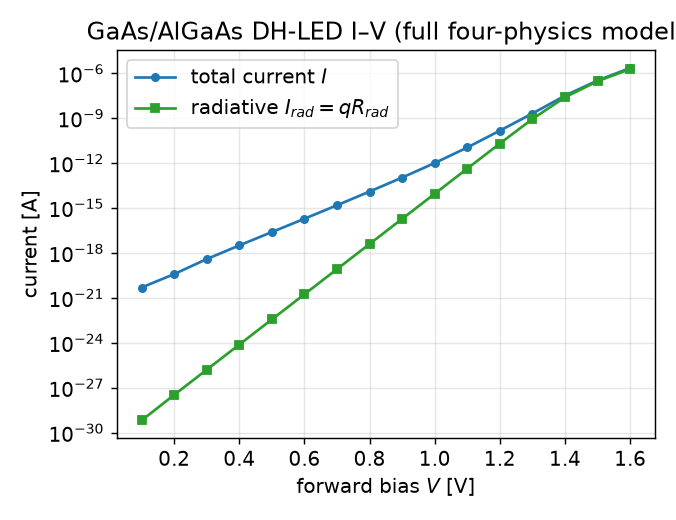
\includegraphics[width=0.92\columnwidth]{fig1_iv.png}
\caption{Total and radiative I--V of the full four-physics model. The radiative
current $I_{\mathrm{rad}}=qR_{\mathrm{rad}}$ approaches the total current as the
device enters efficient injection.}
\label{fig:iv}
\end{figure}

\begin{figure}[t]
\centering
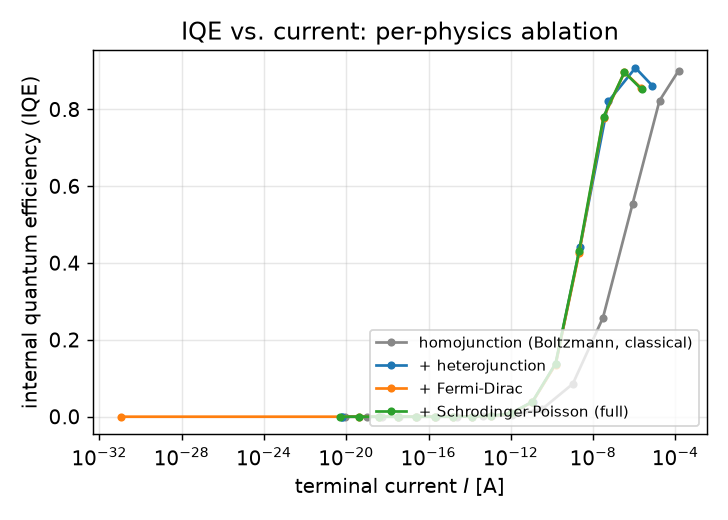
\includegraphics[width=0.98\columnwidth]{fig2_iqe_ablation.png}
\caption{Internal quantum efficiency vs. terminal current for the four
configurations. The heterostructure curves reach a given IQE at $\sim\!10^2\times$
lower current than the homojunction---the double-heterostructure advantage.}
\label{fig:iqe}
\end{figure}

\begin{figure}[t]
\centering
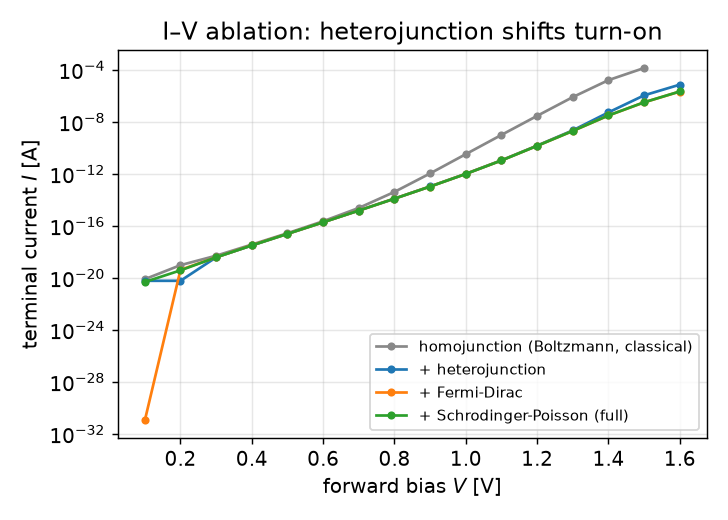
\includegraphics[width=0.98\columnwidth]{fig3_iv_ablation.png}
\caption{I--V ablation. The heterojunction band offsets raise the barrier and
shift the current turn-on.}
\label{fig:ivabl}
\end{figure}

\begin{figure*}[t]
\centering
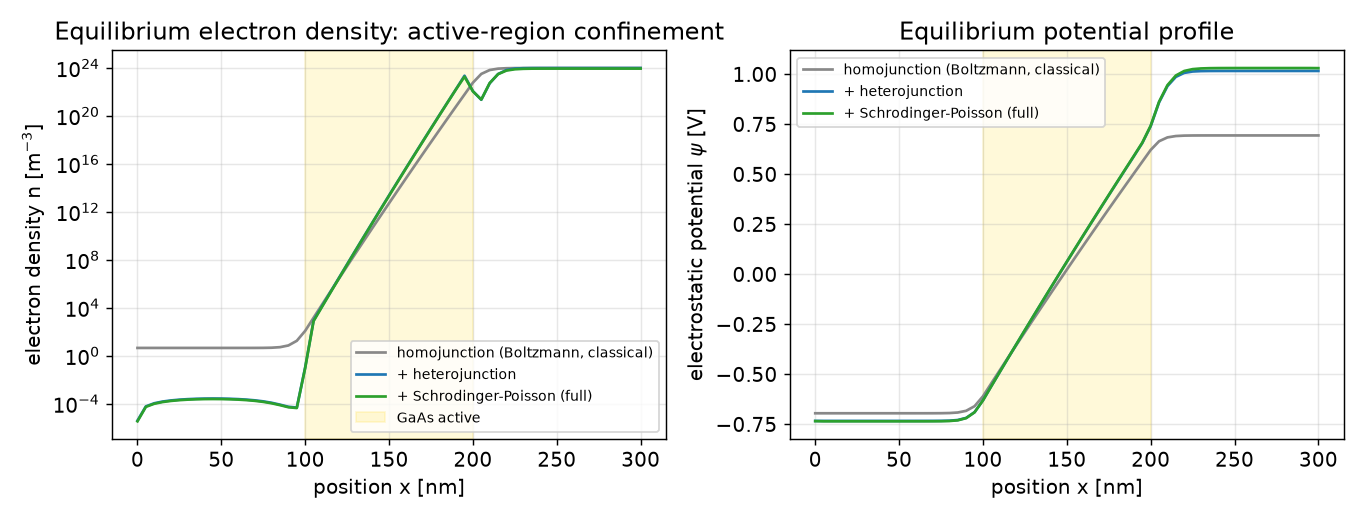
\includegraphics[width=0.86\textwidth]{fig4_confinement.png}
\caption{Equilibrium electron density (left) and electrostatic potential (right)
across the device for the homojunction, heterojunction and full Schr\"odinger--Poisson
model. The GaAs active region (100--200\,nm) is shaded. The full-model density
peak is set back from the heterointerface by the quantum correction.}
\label{fig:conf}
\end{figure*}

\begin{figure}[t]
\centering
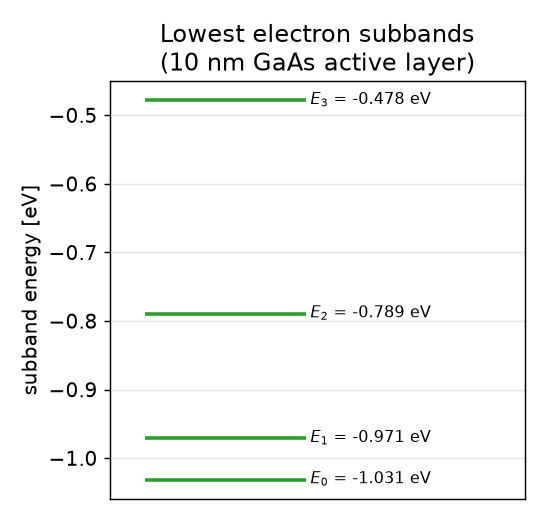
\includegraphics[width=0.62\columnwidth]{fig5_subbands.png}
\caption{The four lowest confined electron subbands resolved by the
self-consistent Schr\"odinger--Poisson loop in the $10\,$nm GaAs active layer.}
\label{fig:sub}
\end{figure}

\section{Validation}
The solver is checked against analytic semiconductor physics by a unit-test suite
($\approx110$ tests): the built-in potential matches
$V_{bi}=V_T\ln(N_A N_D/n_i^2)$ for the homojunction; mass action $np=n_i^2$ holds
at equilibrium to machine precision; the forward I--V is rectifying and
exponential with ideality factor $\approx1$; and the terminal currents at the two
contacts are equal and opposite (conservation). The recombination Jacobian
derivatives match finite differences; the classical limit ($\Lambda=0$, Boltzmann)
is byte-for-byte identical to the pure DD solver; the SP subband eigenvalues come
out ascending and the self-consistent loop converges with a bounded quantum
potential while conserving charge; and the optical read-out gives
$\mathrm{IQE}\in(0,1]$ with the emission wavelength matching the active-region gap
and $I_{\mathrm{rad}}=qR_{\mathrm{rad}}$. These checks establish that the coupled
four-physics result rests on individually-verified components.

\section{Conclusion and Future Work}
We have demonstrated, in a single open, test-validated 2-D FEM drift-diffusion
solver, the fully-coupled combination of heterojunction electrostatics,
self-consistent Schr\"odinger--Poisson subband confinement, Fermi--Dirac
degeneracy and radiative recombination for a GaAs/AlGaAs double-heterostructure
LED, and we have attributed the change each effect produces through a controlled
per-physics ablation. The heterojunction raises the built-in potential and shifts
the turn-on so the DH device reaches a given IQE at $\sim\!100\times$ lower
current; Fermi--Dirac corrects the degenerate-cladding over-count; the SP loop
resolves the active-layer subbands and redistributes the confined carriers; and
the radiative channel yields a peak IQE of $0.90$ at $873\,$nm. The combination---%
open, reproducible, and coupling a genuine self-consistent SP correction rather
than a density-gradient surrogate---fills a gap between closed commercial TCAD and
existing open device simulators.

Future work follows two directions in the solver roadmap: heterointerface
thermionic-emission transport (HBTs/HEMTs) and GaN polarization charge (nitride
emitters), extending the framework to visible and UV LEDs; and, as a distinct
study, adapting the transport and recombination machinery---with field/density
dependent (EGDM) mobility and Gauss--Fermi statistics---toward organic and
quantum-dot LEDs.

\section*{Reproducibility}
All numbers and figures regenerate from the scripts in \texttt{code/}
(\texttt{ablation.py}, \texttt{make\_figs.py}) against the open DDM.SPC solver; the
raw ablation data is in \texttt{data/ablation.json} and the figures in
\texttt{figures/}.

\begin{thebibliography}{9}
\bibitem{alferov} Zh.~I.~Alferov, ``Nobel Lecture: The double heterostructure
concept and its applications,'' \emph{Rev. Mod. Phys.}, vol.~73, no.~3,
pp.~767--782, 2001.
\bibitem{devsim} J.~E.~Sanchez and R.~Ananian-Cooper, ``DEVSIM: A TCAD
Semiconductor Device Simulator,'' \emph{J. Open Source Software}, vol.~7, no.~70,
3898, 2022.
\bibitem{genius} Cogenda Pte. Ltd., ``Genius-TCAD-Open: Open-source edition of the
Genius Semiconductor Device Simulator.'' [Online]. Available:
\url{https://github.com/cogenda/Genius-TCAD-Open}
\bibitem{charon} Sandia National Laboratories, ``Charon: A drift-diffusion /
hydrodynamic semiconductor device simulation code.'' [Online]. Available:
\url{https://charon.sandia.gov}
\bibitem{semidv} ``SEMIDV: A Compact Semiconductor Device Simulator with Quantum
Effects,'' arXiv:2504.00214, 2025.
\bibitem{qdd} C.~de~Falco, E.~Gatti, A.~L.~Lacaita, and R.~Sacco, ``Quantum-corrected
drift-diffusion / coupled Schr\"odinger--drift-diffusion models for quantum
semiconductor device simulations,'' \emph{J. Comput. Phys.}, vol.~176,
pp.~149--166, 2002.
\bibitem{demari} A.~De~Mari, ``An accurate numerical steady-state one-dimensional
solution of the p-n junction,'' \emph{Solid-State Electron.}, vol.~11,
pp.~33--58, 1968.
\bibitem{bednarczyk} D.~Bednarczyk and J.~Bednarczyk, ``The approximation of the
Fermi--Dirac integral $F_{1/2}(\eta)$,'' \emph{Phys. Lett. A}, vol.~64, no.~4,
pp.~409--410, 1978.
\bibitem{gummel} H.~K.~Gummel, ``A self-consistent iterative scheme for
one-dimensional steady state transistor calculations,'' \emph{IEEE Trans.
Electron Devices}, vol.~11, pp.~455--465, 1964.
\end{thebibliography}

\vspace{2mm}
\footnotesize\emph{Note:} bibliographic details for \cite{charon}, \cite{qdd},
\cite{demari}, \cite{bednarczyk}, \cite{gummel} should be verified against the
primary sources before camera-ready submission.

\end{document}
